\chapter{Experiments and Results}

\par Every collaborative task previously described was successfully implemented, but in order to validate its quality, performance and accuracy, a series of experiments were created. They consist on quantitative and qualitative metrics and serve as a benchmark of the techniques and tasks developed in this Dissertation.

\section{Collaborative Setup}

\par The experimental setup consists on a \ac{ur10e}, with a Weiss Robotics CRG 200 gripper attachment. The vision sensor is a Microsoft Kinect \acs{rgbd} camera and the shared workspace is a simple table, approximately 50cm distant from the robot. The camera is positioned at 2m of height with a \ang{45} downwards orientation and its \ac{fov} is shown in \autoref{fig:kinect}. The complete composition of the setup is described in \autoref{fig:setup}.

\begin{figure}[h]
    \centering
    \begin{subfigure}{.5\textwidth}
      \centering
      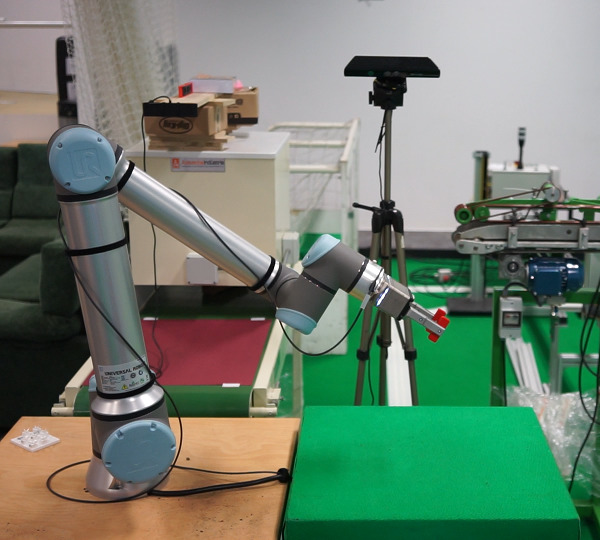
\includegraphics[width=.9\linewidth]{figs/chp6/setup.jpg}
      \caption{Setup View}
      \label{fig:setup}
    \end{subfigure}%
    \begin{subfigure}{.5\textwidth}
      \centering
      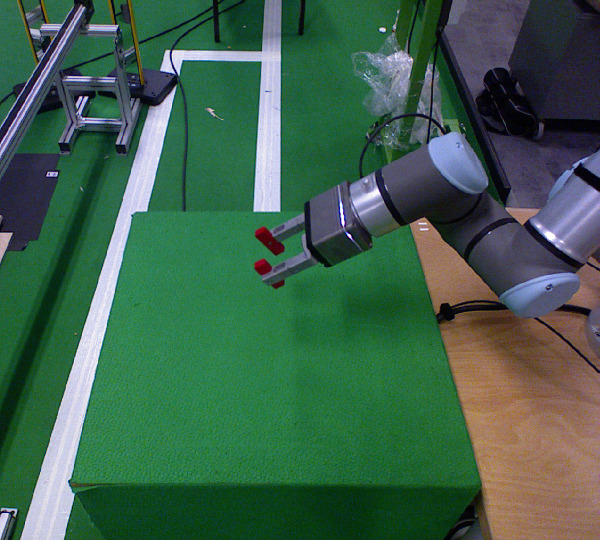
\includegraphics[width=.9\linewidth]{figs/chp6/kinect.jpg}
      \caption{Kinect View}
      \label{fig:kinect}
    \end{subfigure}
    \caption{Views of the experimental shared workspace}
    \label{fig:setup_and_kinect}
    \end{figure}

\section{Execution of the collaborative tasks}

\subsection{Interaction Test}

\par To validate the use of the \ac{eef} double tap as an interaction interface with the cobot, a test case was developed in which the user would make consecutive double taps in all the directions available and observe if they were correctly registered through the colors of the gripper \acsp{led}. Each direction corresponds to a different color. A double tap interaction is considered a fail when the color of the \acsp{led} does not change, or changes to the wrong color.

\begin{table}[h]
    \centering
    \begin{tabular}{|c|c|c|}
    \hline
    \textbf{Double Taps} & \textbf{Fails} & \textbf{Accuracy} \\ \hline
    300 & 16 & 94,6\% \\ \hline
    \end{tabular}
    \caption{Results of the interaction test}
    \label{tab:interaction_test}
\end{table}

\par In 300 interactions, 94,5\% were correctly registered. Between the fails, the majority were due to weak execution of the double tap. There was record of a few interactions in which the direction was wrongly classified. The cause of this is due to the ambiguous direction in which the user performed the double tap.

\subsection{Hand Guiding}

\par The accuracy of the \ac{eef} compensation model was already discussed in \autoref{ssec:ft_theory_model}. It has been proved that a force threshold of 2N would be possible since it is higher than the maximum error of the \ac{ft} theoretical model. Despite this fact, it has also been shown in \autoref{ssec:ft_sensor_behavior} that physical interaction with the sensor can cause deviations in its measurements. For this reason, an experimental test was developed to test the accuracy of the compensation model in a real scenario, and the performance of the \ac{hg} task in general.

\begin{figure}[h]
    \centering
    \begin{subfigure}{.2\linewidth}
        \centering
        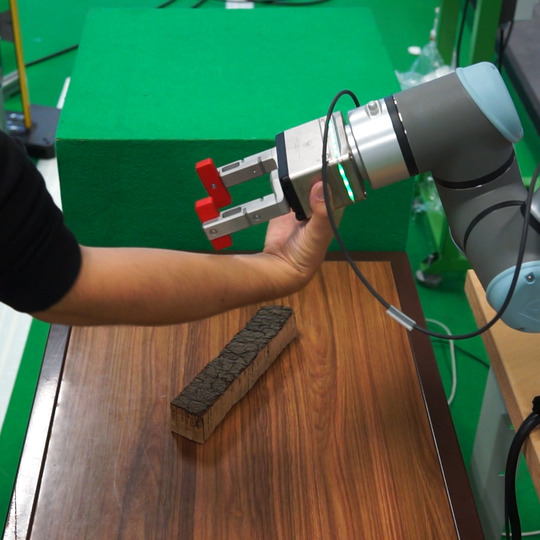
\includegraphics[width=.95\linewidth]{figs/chp6/hg_test_0.jpg}
    \end{subfigure}%
    \begin{subfigure}{.2\linewidth}
        \centering
        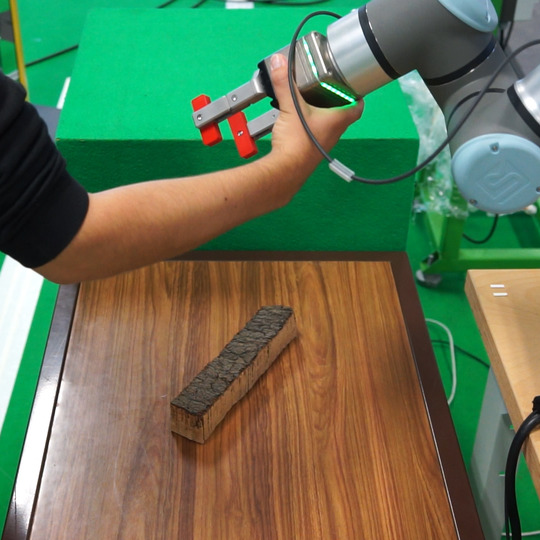
\includegraphics[width=.95\linewidth]{figs/chp6/hg_test_1.jpg}
    \end{subfigure}%
    \begin{subfigure}{.2\linewidth}
        \centering
        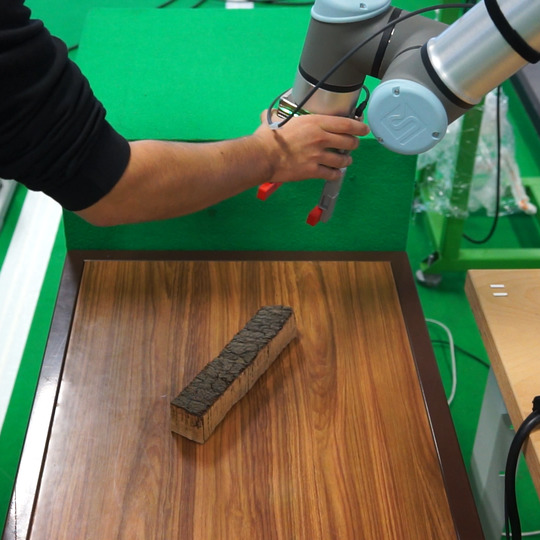
\includegraphics[width=.95\linewidth]{figs/chp6/hg_test_2.jpg}
    \end{subfigure}%
    \begin{subfigure}{.2\linewidth}
        \centering
        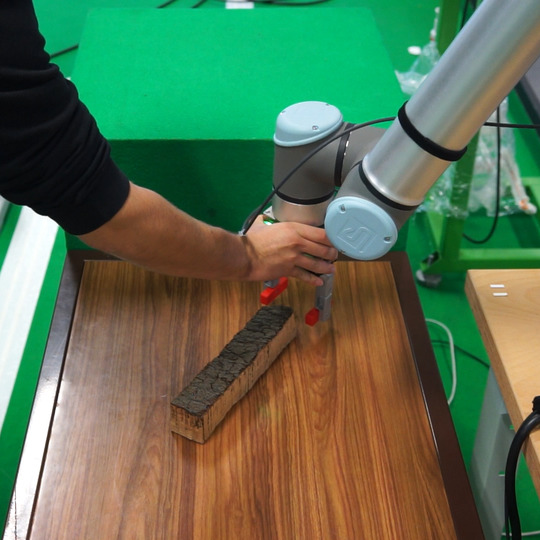
\includegraphics[width=.95\linewidth]{figs/chp6/hg_test_3.jpg}
    \end{subfigure}%
    \begin{subfigure}{.2\linewidth}
        \centering
        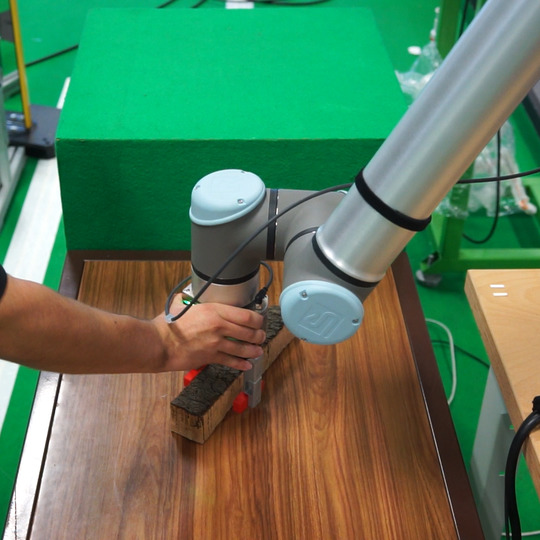
\includegraphics[width=.95\linewidth]{figs/chp6/hg_test_4.jpg}
    \end{subfigure}
    \caption{Succession of steps of the \ac{hg} test}
    \label{fig:hg_test}
\end{figure}

\par The test consists on rapidly \ac{hg} the cobot from a start position, to a random position in the workspace. This first step serves to test the responsiveness and ease of use of the system. Then, the user must align the gripper fingers with an object that is placed on the table. The system must compensate the \ac{ft} caused by the gripper in every orientation, therefore the cobot must only move due to external forces caused by the user. On the other hand, the user must align the gripper fingers with the object without difficulty. This test was performed 10 times in multiple settings of force thresholds from the compensation model. 


\begin{table}[h]
    \centering
    \begin{tabular}{|c|c|c|c|}
    \hline
    \textbf{\begin{tabular}[c]{@{}c@{}}Compensation\\ Threshold\end{tabular}} & \textbf{\begin{tabular}[c]{@{}c@{}}Test\\ Accuracy\end{tabular}} & \textbf{\begin{tabular}[c]{@{}c@{}}Test\\ Responsiveness\end{tabular}} & \textbf{\begin{tabular}[c]{@{}c@{}}Qualitative\\ Performance\end{tabular}} \\ \hline
    \textbf{1N} & 3/10 & 10/10 & Unusable \\ \hline
    \textbf{2N} & 8/10 & 10/10 & Usable \\ \hline
    \textbf{3N} & 10/10 & 10/10 & Balanced \\ \hline
    \textbf{4N} & 10/10 & 8/10 & Satisfactory \\ \hline
    \textbf{5N} & 10/10 & 5/10 & Unresponsive \\ \hline
    \end{tabular}
    \caption{Results of the \ac{hg} performance test}
    \label{tab:hand_guiding_test}
\end{table}

% ADD: Definir bem o que é Accuracy and Responsiveness (se calhar mudar as definições)

\par The results are outlined in \autoref{tab:hand_guiding_test} and below is a detailed description of their meaning:
\begin{itemize}
    \item At 1N of force threshold, the system is unusable. The cobot is mostly moving by itself since the force threshold is too low. This result is expected and serves as a demonstration of the consequences of the inaccuracies of the \ac{ft} sensor.
    \item At 2N, the accuracy results are improved, but not entirely satisfactory. Due to physical interaction with the sensor, there were certain motions that would cause deviations on the \ac{ft} measurements. Despite this fact, with this setting the cobot is very responsive, reacting to very low amounts of force and allowing the gripper to be easily placed exactly where the user wants it to be.
    \item 3N proved to be the best threshold setting. It allowed the correct execution of every test and the loss on responsiveness was not perceptible. With this gripper attachment, 3N will be the default value for force threshold on the \ac{eef} weight compensation model.
    \item 4N and 5N allowed the same accuracy results obtained with 3N but at the cost of motion responsiveness. In short, the user would have to exert higher amounts of force on the \ac{eef} for it to move, causing degradation on its smoothness.
\end{itemize}

\par In terms of general execution of the \ac{hg} task...

\subsection{Object Manipulation}

\par The object manipulation task requires the dynamic attachment of extra weight to the cobot \ac{eef}. It has been showed previously that the \ac{eef} weight compensation model supports dynamic changing of the weight and \ac{cog} parameter, but the performance of this manipulation task is directly proportional to the accurate measurement of this parameters.
\par The first test regarding this task should be to find both system and \ac{ft} sensor performance on correctly measuring the weight of the coupled object. In order to do this a 1Kg iron weight will be gripped by the cobot 10 times in 4 different orientations. The first 3 orientations consist on vertically aligning each force axis with gravity in order to obtain the accuracy of each measurement component. The last orientation consist on a set of rotations in order for the weight to be distributed evenly in the 3 axis.

% ADD: Photos of the positions

\par Show weight tests..

% ADD: Weight plots

\par Present results form the weight tests... 

\par Assuming the weight is correctly obtained, a real time test was performed to demonstrate that the \ac{eef} weight compensation model can sustain the same levels of accuracy independent of the weight coupled to the robot. \autoref{fig:object_result} shows a real time test where Wrist1 and Wrist2 joints are rotated causing multiple \ac{eef} orientations. Similar to previous real time tests the \ac{eef} weight is compensated with minimal error.

\begin{figure}[h]
    \centering
    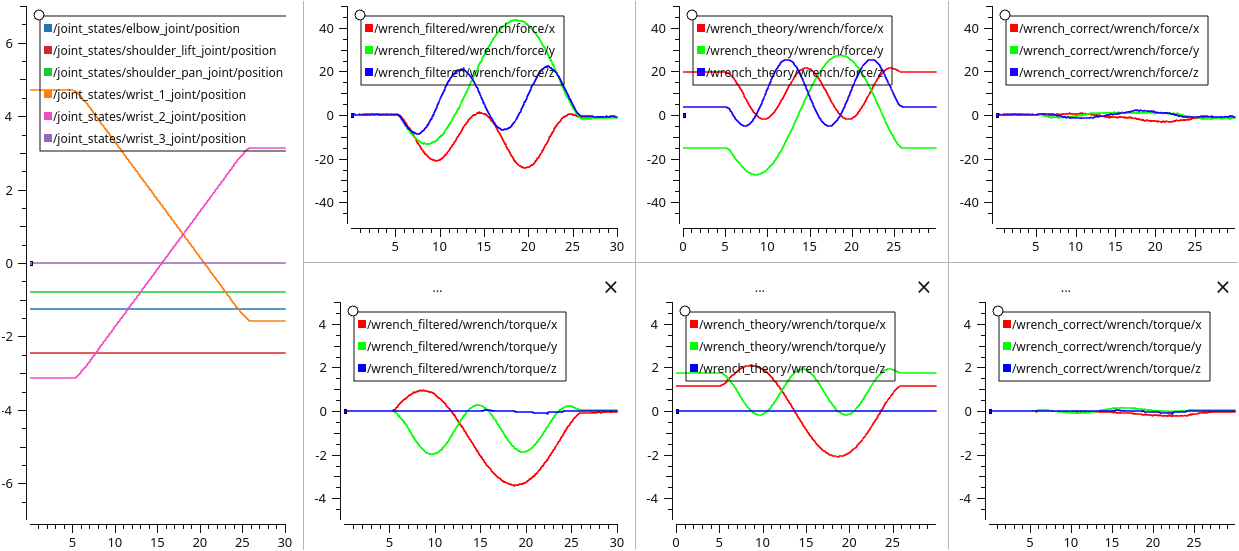
\includegraphics[width=0.9\linewidth]{figs/chp6/object_result.png}
    \caption{Result of the compensation architecture applied in a real time test}
    \label{fig:object_result}
\end{figure}

\begin{figure}[h]
    \centering
    \begin{subfigure}{.2\linewidth}
        \centering
        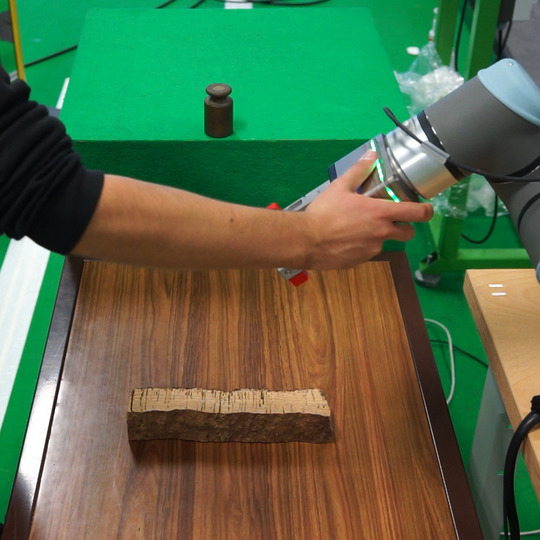
\includegraphics[width=.95\linewidth]{figs/chp6/om_test_0.jpg}
    \end{subfigure}%
    \begin{subfigure}{.2\linewidth}
        \centering
        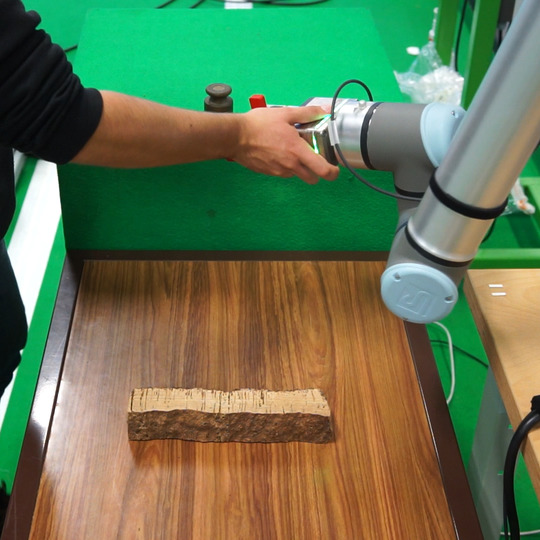
\includegraphics[width=.95\linewidth]{figs/chp6/om_test_1.jpg}
    \end{subfigure}%
    \begin{subfigure}{.2\linewidth}
        \centering
        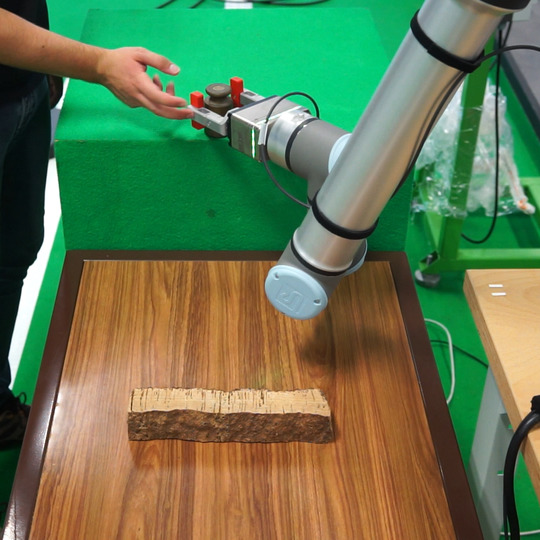
\includegraphics[width=.95\linewidth]{figs/chp6/om_test_2.jpg}
    \end{subfigure}%
    \begin{subfigure}{.2\linewidth}
        \centering
        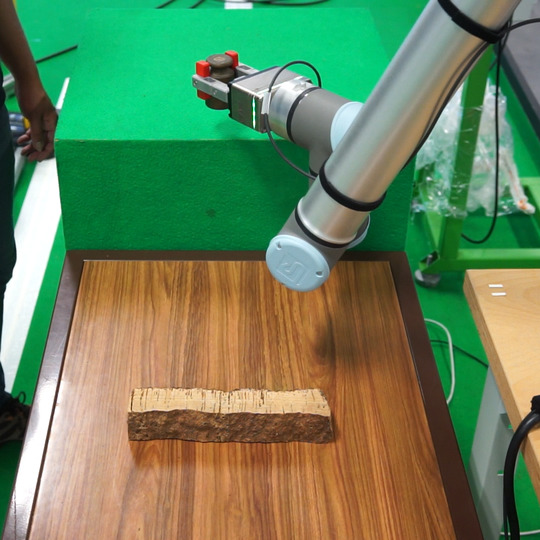
\includegraphics[width=.95\linewidth]{figs/chp6/om_test_3.jpg}
    \end{subfigure}%
    \begin{subfigure}{.2\linewidth}
        \centering
        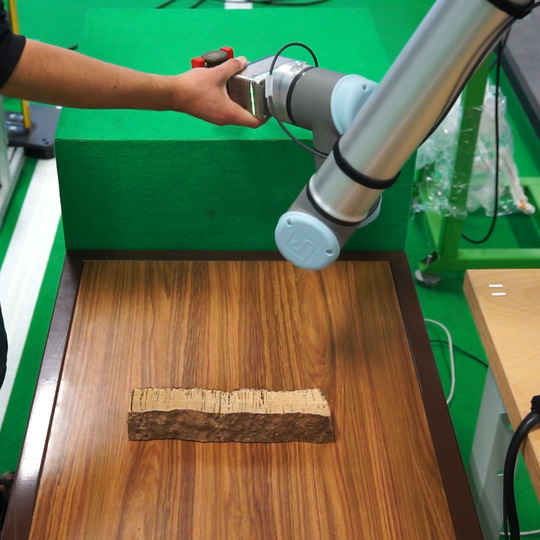
\includegraphics[width=.95\linewidth]{figs/chp6/om_test_4.jpg}
    \end{subfigure}
    \par\smallskip
    \begin{subfigure}{.2\linewidth}
        \centering
        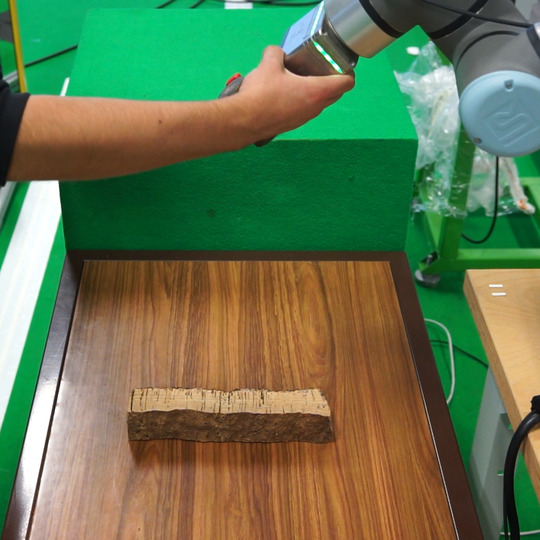
\includegraphics[width=.95\linewidth]{figs/chp6/om_test_5.jpg}
    \end{subfigure}%
    \begin{subfigure}{.2\linewidth}
        \centering
        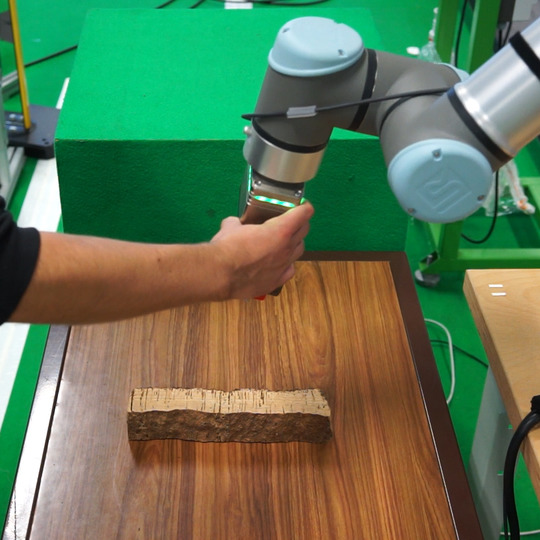
\includegraphics[width=.95\linewidth]{figs/chp6/om_test_6.jpg}
    \end{subfigure}%
    \begin{subfigure}{.2\linewidth}
        \centering
        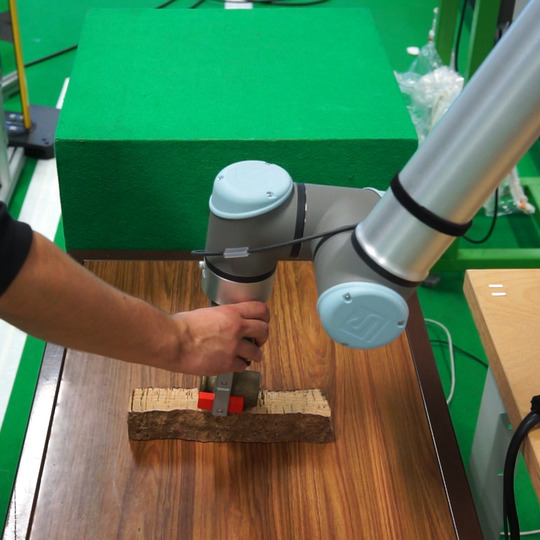
\includegraphics[width=.95\linewidth]{figs/chp6/om_test_7.jpg}
    \end{subfigure}%
    \begin{subfigure}{.2\linewidth}
        \centering
        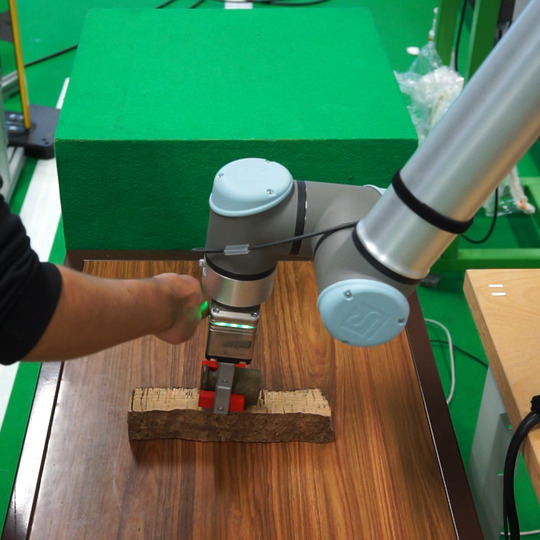
\includegraphics[width=.95\linewidth]{figs/chp6/om_test_8.jpg}
    \end{subfigure}%
    \begin{subfigure}{.2\linewidth}
        \centering
        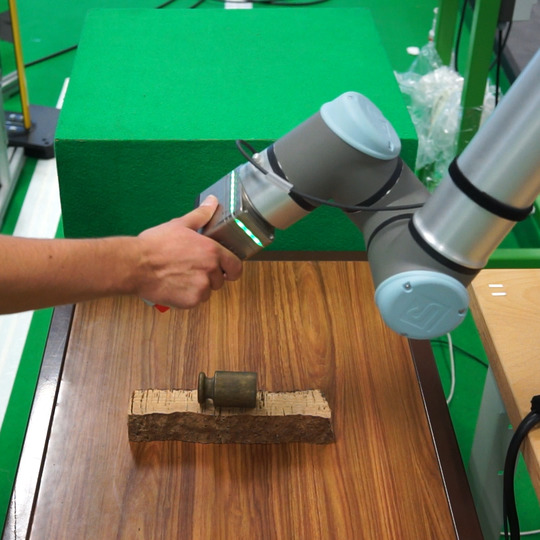
\includegraphics[width=.95\linewidth]{figs/chp6/om_test_9.jpg}
    \end{subfigure}
    \caption{Succession of steps of the object manipulation test}
    \label{fig:om_test}
\end{figure}

\par For the same reasons as in the \ac{hg} tests, weight compensation error is not enough to validate this task. Furthermore, since extra weight is added, it is suspected that the deviations caused by physical interaction with the \ac{ft} sensor will increase compared to the previous task. This time, the collaborative test consists on \ac{hg} the cobot in order to grab a stationary object in the environment, order it to grip it, wait for it to calibrate its payload and manipulate the object casing both linear and angular movements in order to release it at another location in the environment. The test was also repeated 10 times in each force threshold setting.

\begin{table}[h]
    \centering
    \begin{tabular}{|c|c|c|c|}
    \hline
    \textbf{\begin{tabular}[c]{@{}c@{}}Compensation\\ Accuracy\end{tabular}} & \textbf{\begin{tabular}[c]{@{}c@{}}Test\\ Accuracy\end{tabular}} & \textbf{\begin{tabular}[c]{@{}c@{}}Test\\ Responsiveness\end{tabular}} & \textbf{\begin{tabular}[c]{@{}c@{}}Qualitative\\ Performance\end{tabular}} \\ \hline
    \textbf{1N} & 0/10 & 10/10 & Unusable \\ \hline
    \textbf{2N} & 3/10 & 10/10 & Unusable \\ \hline
    \textbf{3N} & 7/10 & 10/10 & Usable \\ \hline
    \textbf{4N} & 9/10 & 8/10 & Satisfactory \\ \hline
    \textbf{5N} & 10/10 & 5/10 & Unresponsive \\ \hline
    \end{tabular}
    \caption{Results of the object manipulation performance test}
    \label{tab:object_manipulation_test}
\end{table}

\par \autoref{tab:object_manipulation_test} presents the results of the test and similar to the previous task an interpretation of them will follow: 
\begin{itemize}
    \item Similar to the \ac{hg} task and for the same reason, 1N of force threshold is unusable.
    \item \textbf{Continuar...}
\end{itemize}

\par explain why responsiveness is bad when incresing weight, cuz robot doenst know the payload and the motions are jerky

\par explian that by rasing the force threshlod it solves the issue, and threshold should be raised proportionally to the weight, say that is possible maintain a ratio of 1:5 in this scenario but with a more accurate sensor 1:10 is possible

\subsection{Collision Avoidance}

\par Make a XYZ graph with the predefined trajectory and the collision avoidance trajectory
\par Make a table with varying number of objects and benchmark completeness
\par Make a table with the response times of hte object detection (gazebo)

\section{System Stability}

\par explain that the robot is always stoping and complaining because payload is not set... explain that payload cannot be set... explain how to solve this issue such has the use of an external sensor